\subsection{\label{subsec:massivenus_whereweare}Current knowledge of neutrino mass and mixing}
%
Neutrinos are the lightest known elementary fermions. They do not carry electric or color charge, and are observable only via weak interactions. In the Standard Model (SM) of elementary particles, neutrinos are paired with charged leptons in weak isodoublets. Experimentally, we know that only three light ---\thinspace that is, of mass smaller than $m_Z/2$, where $m_Z$ is the mass of the $Z$ boson\thinspace--- \emph{active} neutrino families exist.

Neutrino oscillation experiments at the turn of the millennium unambiguously demonstrated that neutrinos are massive particles \cite{Super-Kamiokande:1998kpq,SNO:2001kpb,SNO:2002tuh}. Because of the interferometric nature of neutrino oscillations, such experiments can only measure squared-mass differences and not the absolute neutrino mass scale. Solar and reactor experiments have measured one mass difference, the so-called \emph{solar mass splitting}, to be: $\Delta m^2_{21}\equiv m^2_2-m^2_1= (7.41^{+0.21}_{-0.20})\times 10^{-5}\ {\rm eV}^2$. Atmospheric and accelerator-based experiments have measured a different mass splitting, the so-called \emph{atmospheric mass splitting}, to be: $\lvert\Delta m^2_{\rm 31}\rvert\equiv \lvert m^2_3-m^2_1\rvert= (2.511^{+0.028}_{-0.027})\times 10^{-3}\ {\rm eV}^2\gg \Delta m^2_{21}$. In the standard 3-neutrino oscillations' paradigm, those are the only two independent mass splittings available. The best-fit values and 1$\sigma$ ranges quoted were obtained from a recent global 3-neutrino fit \cite{Esteban:2020cvm}. Similar results are obtained in other global analyses \cite{deSalas:2020pgw,Capozzi:2021fjo}.

The observation of neutrino flavor oscillations also imply that the neutrino states participating in the weak interactions (\emph{flavor eigenstates}) are different from the neutrino states controlling free particle evolution (\emph{mass eigenstates}). In other words, the three weak eigenstates $\lvert\nu_{\alpha}\rangle,\ \alpha=e,\mu,\tau$, can be expressed as a linear combination of the three mass eigenstates $\lvert\nu_{i}\rangle,\ i=1,2,3$:
%
\begin{equation}
\lvert \nu_{\alpha}\rangle = \sum_i U_{\alpha i}^{\ast}\lvert \nu_i\rangle
\label{eq:neutrinomixing}
\end{equation}
%
\noindent where $U$ is a $3\times3$, unitary, \emph{neutrino mixing matrix}, that is different from unity. Equation \ref{eq:neutrinomixing} implies the violation of the individual lepton flavors $L_{\alpha}$, but not necessarily the violation of the total lepton number $L\equiv \sum_{\alpha} L_{\alpha} = L_e+L_{\mu}+L_{\tau}$. The $3\times 3$ neutrino mixing matrix is usually parametrized in terms of 3 Euler angles $(\vartheta_{12},\ \vartheta_{13},\ \vartheta_{23})$ and 3 phases $(\delta,\ \alpha_{21},\ \alpha_{31})$ (see, for example, \cite{ParticleDataGroup:2022pth}). If the massive neutrinos are \emph{Dirac particles} (see sect.~\ref{subsec:massivenus_identity}), only the \emph{Dirac phase} $\delta$ is physical and can be responsible for CP violation in the lepton sector. If the massive neutrinos are \emph{Majorana particles} (sect.~\ref{subsec:massivenus_identity}), the two additional \emph{Majorana phases} $(\alpha_{21},\ \alpha_{31}$) are also potentially observable.

Neutrino oscillation experiments have measured with few percent-level accuracy the flavor content of the neutrino mass states participating in 3-neutrino mixing. Atmospheric and accelerator-based neutrino oscillation experiments are mostly driven by $\nu_{\mu}\to\nu_{\tau}$ oscillations, with a sub-leading yet well-established $\nu_{\mu}\to\nu_{e}$ oscillation component.  They have therefore measured the muon and tau flavor contents of the $\nu_3$ mass state to be large and similar among them ($\lvert U_{\mu 3}\rvert^2\simeq \lvert U_{\tau 3}\rvert^2\simeq 0.5$), and that such mass state has little electron flavor content ($\lvert U_{e3}\rvert^2\simeq 0.02$). On the other hand, solar and reactor neutrino oscillation experiments are consistent with $\nu_e\to\nu_{\mu}$ and $\nu_e\to\nu_{\tau}$ transitions. They have measured $\lvert U_{e2}\rvert^2\simeq 0.3$. The remaining elements of the leptonic mixing matrix can  be derived, given $(\lvert U_{\mu 3}\rvert,\lvert U_{e3}\rvert,\lvert U_{e2}\rvert)$, assuming unitarity. More precisely, according to \cite{Esteban:2020cvm}, the 3$\sigma$ ranges in the magnitude of the elements of the three-flavor leptonic mixing matrix under the assumption that the matrix U is unitary are:
 %
\begin{equation}
  \label{eq:umatrix}
  \begin{aligned}
    \lvert U\rvert_{3\sigma} &=
    \begin{pmatrix}
      0.803 \to 0.845 &\qquad
      0.514 \to 0.578 &\qquad
      0.143 \to 0.155
      \\
      0.244 \to 0.498 &\qquad
      0.502 \to 0.693 &\qquad
      0.632 \to 0.768
      \\
      0.272 \to 0.517 &\qquad
      0.473 \to 0.672 &\qquad
      0.623 \to 0.761
    \end{pmatrix}
  \end{aligned}
\end{equation}
%

The three outstanding unknowns of the 3-neutrino mixing framework that are potentially observable in current and future neutrino oscillation experiments are: the neutrino mass ordering ($m_3>m_1$ or vice versa), the dominant flavor of the $\nu_3$ state ($\lvert U_{\mu 3}\rvert^2 > \lvert U_{\tau 3}\rvert^2$ or vice versa\footnote{This is often called the $\vartheta_{23}$ octant unknown, given that $\lvert U_{\mu 3}\rvert^2 > \lvert U_{\tau 3}\rvert^2$ implies $\vartheta_{23}>\pi/4$, while $\lvert U_{\mu 3}\rvert^2 < \lvert U_{\tau 3}\rvert^2$ implies $\vartheta_{23}<\pi/4$.}), and whether CP violation is violated in the neutrino sector ($\delta\neq 0,\pi$ or not).

Concerning the neutrino mass ordering, current neutrino oscillation results cannot yet differentiate between two possibilities, usually referred to as \emph{normal} and \emph{inverted orderings}. In the former, the gap between the two lightest mass eigenstates corresponds to the small mass difference ($\Delta m^2_{21}$), while in the second case, the gap between the two lightest states corresponds to the large mass difference ($\Delta m^2_{31}$). While we do not know at present whether $\nu_3$ is heavier or lighter than $\nu_1$, we do know that $\nu_2$ is heavier than $\nu_1$, thanks to matter effects affecting the propagation of neutrinos inside the Sun. The exploitation of the same type of matter effect in accelerator-based and atmospheric neutrino experiments should allow us to experimentally establish the neutrino mass ordering in the relatively near future. Future long-baseline neutrino oscillation experiments should also be able to resolve the $\lvert U_{\mu 3}\rvert^2 > \lvert U_{\tau 3}\rvert^2$ ($\vartheta_{23}$ octant) unknown, and to measure leptonic CP violation, provided that the true value of $\delta$ is sufficiently different from 0 and $\pi$. 

The current knowledge on neutrino masses and mixings provided by neutrino oscillation experiments is summarized in fig.~\ref{fig:numass_ordering}. The diagram shows the two possible mass orderings that are compatible with neutrino oscillation data, with increasing neutrino masses from bottom to top. In addition, the electron, muon and tau flavor content of each mass eigenstate is also shown.

%%%%%
\begin{figure}[t!b!]
\begin{center}
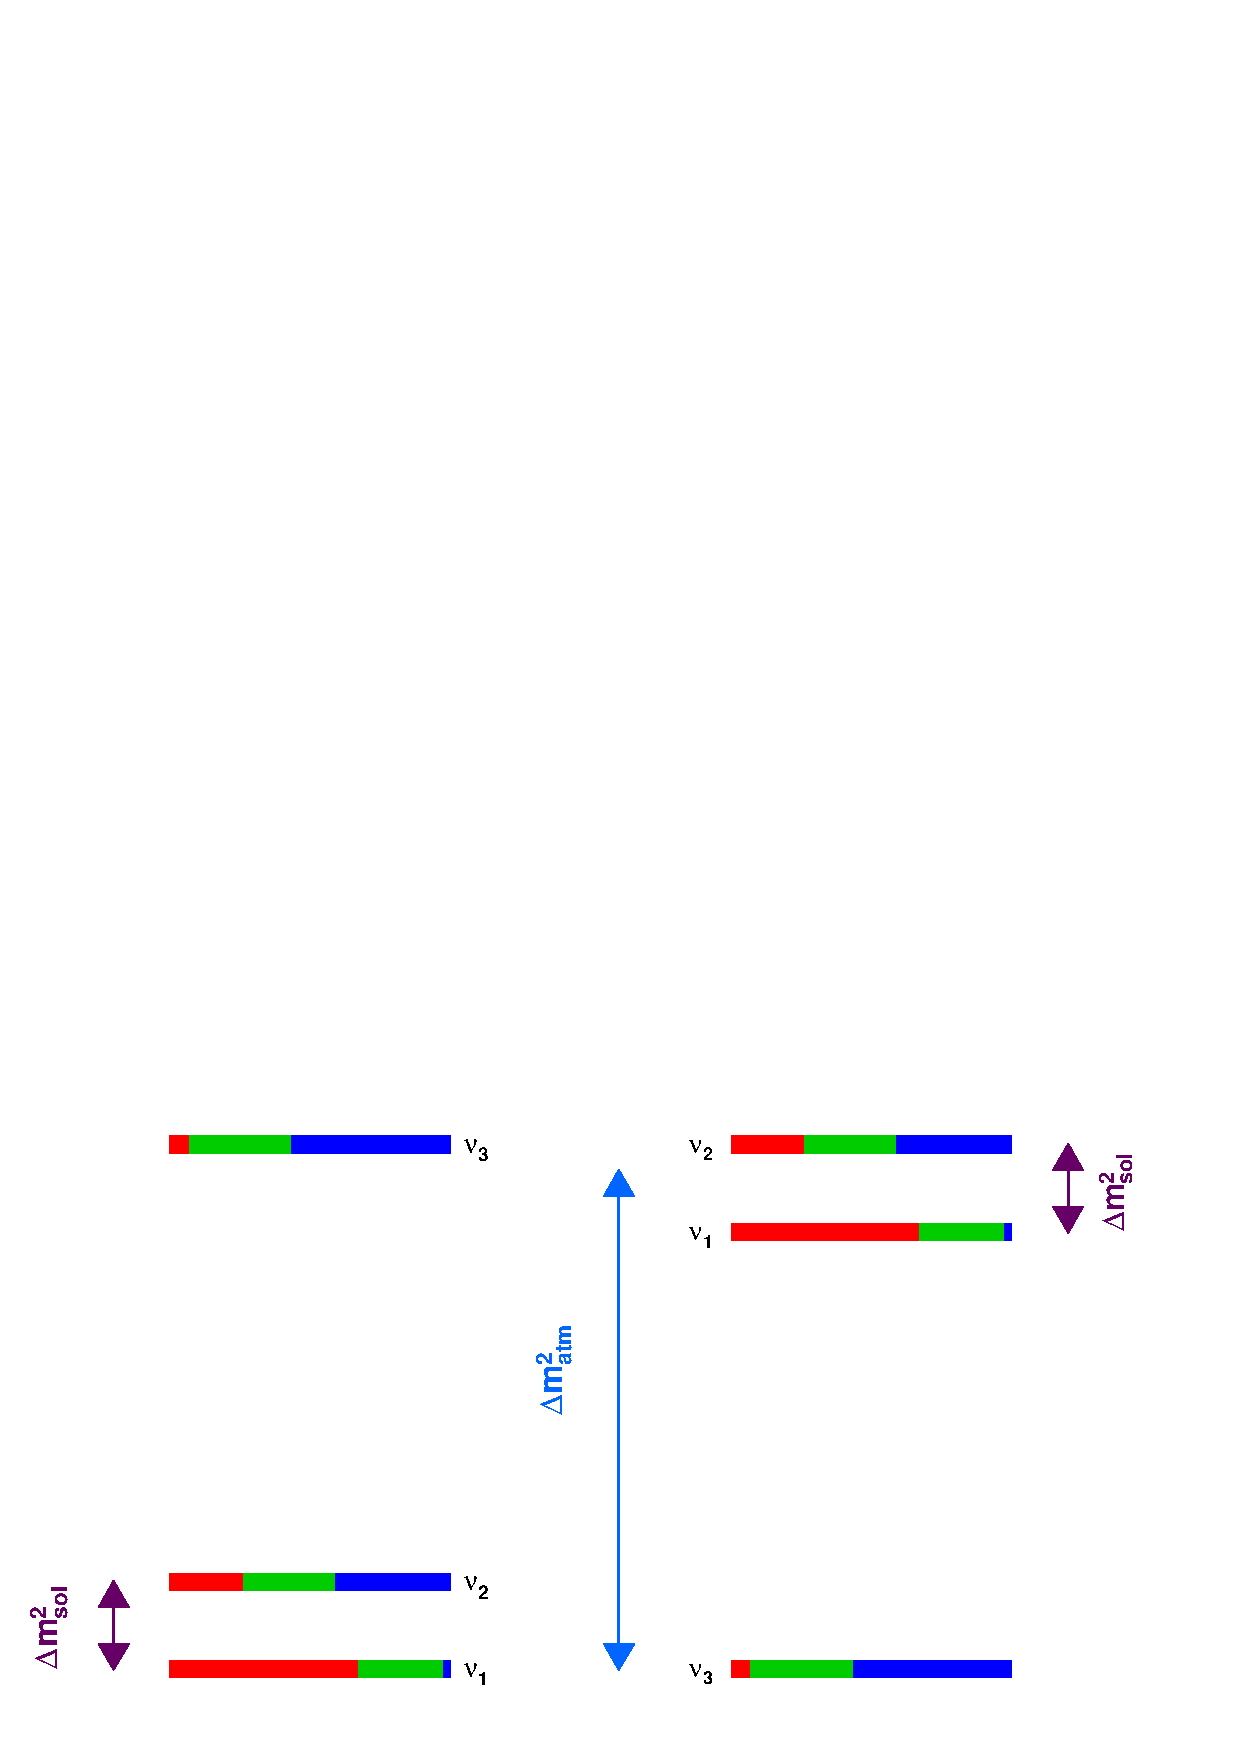
\includegraphics[width=\textwidth]{img/neutrinomassorderings.pdf}
\end{center}
\caption{Probability of finding a certain neutrino flavor in each neutrino mass eigenstate as the CP-violating phase, $\delta$, is
varied.  The left and right panels show the normal (NO) and inverted (IO) mass orderings, respectively. Neutrino masses increase from bottom to top. The electron, muon and tau flavor content of each neutrino mass eigenstate is shown via the blue, red and yellow fractions, respectively. Taken from \cite{DeSalas:2018rby}.}  \label{fig:numass_ordering}
\end{figure}
%%%%%

The absolute value of the neutrino mass scale can instead be probed via neutrinoless double beta decay searches, cosmological observations and beta decay experiments. Only upper bounds on the neutrino mass, of order $\sim$1 eV, currently exist. Constraints on the lightest neutrino mass coming from neutrinoless double beta decay will be discussed in sect.~\ref{subsec:bb0nu_lightmajoranaexchange}. In the following, we briefly summarize cosmological and beta decay constraints.

Primordial neutrinos have a profound impact on cosmology since they affect both the expansion history of the Universe and the growth of perturbations (see, for instance, reference \cite{Lesgourgues:2006nd}). Cosmological observations  can probe the sum of the three neutrino masses:
%
\begin{equation}
m_{{\rm cosmo}}\equiv \sum_{i=1}^3 m_i 
\label{eq:mcosmo}
\end{equation}
% 

Cosmological data are currently compatible with massless neutrinos. Several upper limit values on $m_{{\rm cosmo}}$ can be found in the literature, depending on the details of the cosmological datasets and of the cosmological model that were used in the analysis. A conservative upper limit of $m_{{\rm cosmo}} < 0.13$ eV at 95\% confidence level is obtained when Cosmic Microwave Background (CMB) temperature measurements from the Planck satellite \cite{Planck:2018vyg} are combined with the most recent Baryon Acoustic Oscillation (BAO) measurements from the Sloan Digital Sky Survey (SDSS) galaxy surveys including eBOSS \cite{eBOSS:2020yzd}, in the framework of a Lambda Cold Dark Matter ($\Lambda$CDM) model with dark energy whose equation of state is fixed to $-1$. Even the use of Planck CMB temperature and polarization data alone yields a very robust, and competitive, limit $m_{{\rm cosmo}} < 0.26$ eV at 95\% CL \cite{Planck:2018vyg}.
The relationship between $m_{{\rm cosmo}}$, defined in eq.~(\ref{eq:mcosmo}), and the lightest neutrino mass $m_{{\rm light}}$ ---that is, $m_1$ ($m_3$) in the case of normal (inverted) ordering--- is shown in the top panel of fig.~\ref{fig:mass_constraints_cosmo_beta}. The two bands correspond to the normal and inverted orderings, respectively. The width of the bands is given by the 3$\sigma$ ranges in the mass oscillation parameters $\Delta m^2_{{21}}$ and $\Delta m^2_{{31}}$ \cite{Esteban:2020cvm}. The horizontal band in the top panel of fig.~\ref{fig:mass_constraints_cosmo_beta} is the upper limit on $m_{{\rm cosmo}}$. The $m_{{\rm cosmo}} < 0.13$ eV upper bound translates into a limit of $m_{{\rm light}}\lesssim 0.034\ {\rm eV}$ at 95\% CL in the normal ordering case, as shown by the vertical dashed line in the top panel of fig.~\ref{fig:mass_constraints_cosmo_beta}, and into an even stricter $m_{{\rm light}}$ bound in the inverted ordering case.

%%%%%
\begin{figure}[t!b!]
\begin{center}
\includegraphics[width=0.7\textwidth]{img/mcosmovsmlight.png} 
\includegraphics[width=0.7\textwidth]{img/mbetavsmlight.png}
\end{center}
\caption{\label{fig:mass_constraints_cosmo_beta}Constraints on the lightest neutrino mass $m_{\rm light}$ coming from cosmological (upper panel) and $\beta$ decay (lower panel) experiments. The red and green bands correspond to the normal and inverted orderings, respectively. The $m_{{\rm cosmo}}$ and $m_{\beta}$ upper bounds in the top and bottom panels are from \cite{eBOSS:2020yzd} and \cite{KATRIN:2021uub}, respectively. They translate into the $m_{{\rm light}}$ upper limits shown via the vertical dashed lines.}
\end{figure}
%%%%%

The neutrino mass scale can also be probed in laboratory-based experiments (see, for example, \cite{Otten:2008zz}). The differential electron energy spectrum in nuclear $\beta$ decay experiments is affected both by the neutrino masses and by the mixings defining the electron neutrino state in terms of mass eigenstates. In this case, the mass combination probed is given by:
%%%%%
\begin{equation}
m_{\beta}^2 \equiv \sum_{i=1}^3 \lvert U_{ei}\rvert^2 m_i^2
\label{eq:mbeta}
\end{equation}
%%%%%

The relationship between $m_{\beta}$ in eq.~(\ref{eq:mbeta}) and $m_{{\rm light}}$ is shown in the bottom panel of fig.~\ref{fig:mass_constraints_cosmo_beta}. Again, the results of a recent global fit to neutrino oscillation data \cite{Esteban:2020cvm} are used to determine the $3\sigma$ bands for both the normal and inverted orderings. From the experimental point of view, the region of interest for the study of neutrino properties is located near the $\beta$ endpoint. The most sensitive searches conducted so far are based upon the decay of tritium, via $^3{\rm H}\to^3{\rm He}^+e^-\bar{\nu}_e$, mostly because of the very low $\beta$ endpoint energy of this element (18.6 keV). As for cosmology, $\beta$ decay searches of neutrino mass have so far yielded negative results. The horizontal band in the bottom panel of fig.~\ref{fig:mass_constraints_cosmo_beta} comes from the KATRIN experiment bound, $m_{\beta}<0.8$ eV at 90\% CL \cite{KATRIN:2021uub}. The resulting constraint on $m_{{\rm light}}$ is less stringent than the cosmological one, $m_{{\rm light}}\lesssim 0.8$ eV at 90\% CL. 

%%%%%%%%%%%%%%%%%%%%%%%%%%%%%%%%%%%%%%%%%%%%%%%%%%%%%%%%%%%%%%%%%%%%%%%%%%

\subsection{\label{subsec:massivenus_identity}The origin of neutrino mass: Dirac \emph{versus} Majorana neutrinos}

Are neutrinos their own antiparticles? If the answer is no, we speak of \emph{Dirac neutrinos}. If the answer is yes, we speak of \emph{Majorana neutrinos}. Both possibilities exist for the neutrino, being electrically neutral and not carrying any other charge-like conserved quantum number. Whether neutrinos are Majorana or Dirac particles depends on the nature of the physics that give them mass, given that the two characters are physically indistinguishable for massless neutrinos.

In the Standard Model, only the negative chirality component $\Psi_L$ of a fermion field $\Psi=\Psi_R+\Psi_L$ is involved in the weak interactions. A negative (positive) chirality field $\Psi_{L(R)}$ is a field that obeys the relations $P_{L(R)}\Psi_{L(R)}=\Psi_{L(R)}$ and $P_{R(L)}\Psi_{L(R)}=0$, where $P_L=(1-\gamma_5)/2$ and $P_R=(1+\gamma_5)/2$ are the positive and negative chiral projection operators. 

For massless neutrinos (see, for example, \cite{Hernandez:2010mi}), only the negative chirality neutrino field $\nu_L$ is needed in the theory, regardless of the Dirac/Majorana nature of the neutrino discussed below, since neutrinos only participate in the weak interactions. This field describes \emph{negative helicity} neutrino states $\lvert\nu_L\rangle$ and \emph{positive helicity} antineutrino states\footnote{As customarily done, we use the subscript ``L'' to denote both negative helicity states $\lvert\nu_L\rangle$ and negative chirality fields $\nu_L$, since the terms left-handed helicity states and left-handed chirality fields are also commonly used. Similarly, we denote positive helicity states and positive chirality fields with the subscript ``R'', as in ``right-handed''.}. The positive and negative helicity states are eigenstates of the helicity operator $h\equiv \vec{\sigma}\cdot\hat{p}$ with eigenvalues $\pm 1/2$, respectively, where $\vec{\sigma}$ is the neutrino spin and $\hat{p}$ the neutrino momentum direction. The fact that $\nu_L$ annihilates particles of negative helicity, and creates antiparticles with positive helicity, is not inconsistent with Lorentz invariance, given that the helicity is the same in any reference frame for a fermion travelling at the speed of light. In the Standard Model with massless neutrinos, positive helicity neutrinos and negative helicity antineutrinos do not exist. As a consequence, and since a negative helicity state transforms into a positive helicity state under the parity transformation, the chiral nature of the weak interaction (differentiating negative from positive chirality) implies that parity is maximally violated in the weak interactions.

For relativistic neutrinos of non-zero mass $m$, the neutrino field participating in the weak interactions has still negative chirality, $\nu_L$, but there are sub-leading corrections to the particle annihilation/creation rules described above. The state $\lvert\nu_L\rangle$ that is annihilated by the negative chirality field $\nu_{L}$ is now a linear superposition of the $-1/2$ and $+1/2$ helicity states. The $+1/2$ helicity state enters into the superposition with a coefficient $\propto m/E$, where $E$ is the neutrino energy, and is therefore highly suppressed. 

Neutrino mass terms can be added to the Standard Model Lagrangian in two ways (see, for example, \cite{Giunti:2003qt}). The first way is in direct analogy to the Dirac masses of quarks and charged leptons, by adding the positive chirality component $\nu_R$ of the Dirac neutrino field, describing predominantly positive helicity neutrino states and predominantly negative helicity antineutrino states that do not participate in the weak interactions:
%
\begin{equation}
\label{eq:diracmassterm}
-\mathcal{L}_D=m_D(\overline{\nu_L}\nu_R+\overline{\nu_R}\nu_L),
\end{equation}
%
where $m_D=y v/\sqrt{2}>0$, $y$ is a dimensionless Yukawa coupling coefficient and $v/\sqrt{2}$ is the vacuum expectation value of the neutral Higgs field after electroweak symmetry breaking. In eq.~(\ref{eq:diracmassterm}), $\nu_L$ and $\nu_R$ are, respectively, the negative and positive chirality components of the neutrino field $\nu$. The chiral spinors $\nu_L$ and $\nu_R$ have only two independent components each, leading to the four independent components in the spinor $\nu$. This is different from the case of massless neutrinos, where only the 2-component spinor $\nu_L$ was needed.

The second way in which neutrino mass terms can be added to the Standard Model Lagrangian is unique to neutrinos. Majorana first realized \cite{Majorana:1937vz} that, for neutral particles, one can remove two of the four degrees of freedom in a massive Dirac spinor by imposing the \emph{Majorana condition}:
%%%%%
\begin{equation}
\nu^c = \nu
\label{eq:majoranacondition}
\end{equation}
%%%%% 
where $\nu^c = C\bar{\nu}^T=C(\gamma^0)^T\nu^{\ast}$ is the CP conjugate of the field $\nu$, $C$ is the charge-conjugation operator, $(\nu_L)^c=(\nu^c)_R$ has positive chirality, and $(\nu_R)^c=(\nu^c)_L$ has negative chirality. This result can be obtained by decomposing both the left-hand and right-hand sides of eq.~(\ref{eq:majoranacondition}) into their chiral components, yielding:
%%%%%
\begin{equation}
\nu_R = (\nu_L)^c
\label{eq:nur}
\end{equation}
%%%%%
and therefore proving that the positive chirality component of the Majorana neutrino field $\nu_R$ is not independent of, but obtained from, its negative chirality counterpart $\nu_L$. By substituting eq.~(\ref{eq:nur}) into the mass term in eq.~(\ref{eq:diracmassterm}), we obtain a \emph{Majorana mass term}:
%%%%%
\begin{equation}
\label{eq:majoranamassterml}
-\mathcal{L}_L= \frac{1}{2}m_L(\overline{\nu_L}(\nu_L)^c+\overline{(\nu_L)^c}\nu_L)
\end{equation}
%%%%%
where $m_L$ is a free parameter with dimensions of mass. This Lagrangian mass term implies the existence of a weak isospin triplet scalar (a Higgs triplet), with a neutral component acquiring a non-vanishing vacuum expectation value after electroweak symmetry breaking. Equation (\ref{eq:majoranamassterml}) represents a mass term constructed from negative chirality neutrino fields alone, and we therefore call it a \emph{negative chirality Majorana mass term}. If positive chirality fields also exist and are independent of negative chirality ones, this is not the only possibility. In this case, we may also construct a second Majorana mass term, a \emph{positive chirality Majorana mass term}:
%%%%%
\begin{equation}
\label{eq:majoranamasstermr}
-\mathcal{L}_R= \frac{1}{2}m_R(\overline{\nu_R}(\nu_R)^c+\overline{(\nu_R)^c}\nu_R)
\end{equation}
%%%%%

In the Standard Model, right-handed fermion fields such as $\nu_R$ are weak isospin singlets. As a consequence, and in contrast with $m_D$ or $m_L$, the mass parameter $m_R$ is therefore not connected to a Higgs vacuum expectation value, and could be arbitrarily high. All three mass term in eqs.~(\ref{eq:diracmassterm}), (\ref{eq:majoranamassterml}) and (\ref{eq:majoranamasstermr}) convert negative chirality states into positive chirality ones\footnote{This is because the charge conjugate of a field with a given chirality, such as the ones appearing in eqs.~\ref{eq:majoranamassterml} and \ref{eq:majoranamasstermr}, always has the opposite chirality.}. Chirality is therefore not a conserved quantity, regardless of the Dirac/Majorana nature of neutrinos. Furthermore, the Majorana mass terms in eqs.~(\ref{eq:majoranamassterml}) and (\ref{eq:majoranamasstermr}) convert particles into their own antiparticles. As stated previously, they are therefore forbidden for all electrically charged fermions because of charge conservation. But not only: processes involving Majorana mass terms violate the Standard Model total lepton number $L\equiv L_e+L_{\mu}+L_{\tau}$ by two units ($\lvert\Delta L\rvert=2$), which is not a good quantum number anymore. 

Which of the mass terms allowed in theory, among $\mathcal{L}_D$, $\mathcal{L}_L$ and $\mathcal{L}_R$ in eqs.~(\ref{eq:diracmassterm}), (\ref{eq:majoranamassterml}) and (\ref{eq:majoranamasstermr}) exist in nature? What are the numerical values of the corresponding coupling constants $m_D$, $m_L$, $m_R$? These questions can in principle be answered experimentally. Majorana and Dirac massive neutrinos will in fact have different Standard Model interactions. Let us consider for now an instructive, albeit unrealistic, scattering experiment, see fig.~\ref{fig:DiracMajoranaNeutrinoInteractions}.

\begin{figure}[t!b!]
\begin{minipage}[t]{0.54\textwidth}
\vspace{0pt}
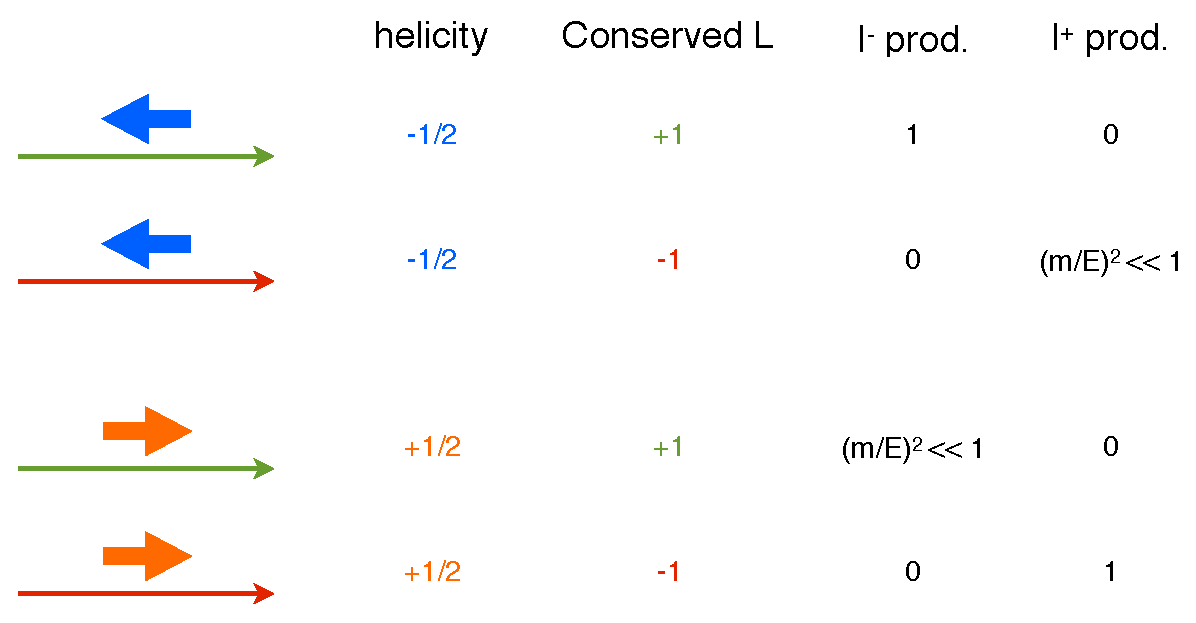
\includegraphics[width=\textwidth]{img/DiracNeutrinoInteraction.eps} % original figure size: 19.69 × 9.99 cm
\end{minipage}
\hfill
\begin{minipage}[t]{0.41\textwidth} % (14.93/19.69)*0.54=0.41
\vspace{0pt}
\includegraphics[width=\textwidth]{img/MajoranaNeutrinoInteraction.eps} % original figure size: 14.93 × 4.73 cm
\end{minipage} 
\caption{The difference between Dirac (left) and Majorana (right) massive neutrinos in a scattering experiment. See text for details. Adapted from \cite{Parke:2010sct}.}
\label{fig:DiracMajoranaNeutrinoInteractions}
\end{figure}

In the Dirac case, Standard Model interactions conserve lepton number $L$, with $L(\nu)=L(l^-)=-L(\bar{\nu})=-L(l^+)=+1$, where $l^{\pm}$ indicates charged leptons. Particles are then identified as neutrinos or antineutrinos in accordance with the process through which they are produced. Charged-current interactions of Dirac neutrinos (as opposed to antineutrinos) produce only $l^-$ and carry a well-defined lepton number $L=-1$, and vice versa. As shown in fig.~\ref{fig:DiracMajoranaNeutrinoInteractions}, for Dirac neutrinos we would thus have four mass-degenerate states: for each of the two available helicity states\footnote{As mentioned above, the weak interaction is maximally parity violating, therefore the two helicity states are distinguishable.}, two distinct particle/antiparticle states characterized by a different $L$ value would be available. Standard Model interactions of neutrino (as opposed to antineutrino) states of positive helicity would have, however, much weaker $l^-$-producing interactions with matter compared to neutrino states of negative helicity, as indicated by the coefficients in fig.~\ref{fig:DiracMajoranaNeutrinoInteractions}. On the other hand, we have seen that in the Majorana case $L$ is not conserved. We would only have two mass-degenerate states, defined by the two available helicity states, see fig.~\ref{fig:DiracMajoranaNeutrinoInteractions}.

Given these differences between Dirac and Majorana massive neutrinos, can we establish which of the two possibilities is realized in Nature via a scattering experiment? In practice, no. The reason is that $l^-$ production from positive helicity Dirac neutrinos (and $l^+$ production from negative helicity Dirac antineutrinos) is expected to be highly suppressed in the ultra-relativisitc limit, and cannot be experimentally observed. Experimentally, all we know is that the neutral particle produced in association with a $l^+$ produces, when interacting, a $l^-$. In the Dirac case, lepton number conservation is assumed, and such neutral particle is identified as the neutrino, with $L=-1$. In the Majorana case, such neutral particle is instead identified as the negative helicity state, interacting differently from its positive helicity counterpart. Both interpretations are viable, and what happens when a neutrino interacts can be understood without invoking a conserved lepton number \cite{Kayser:2002qs}.

Interestingly, the possible observation of the scattering of non-relativistic neutrinos has attracted recent attention. In the non-relativistic case, the difference between Majorana and Dirac neutrinos would become pronounced. The only source of non-relativistic neutrinos known in Nature is the Cosmic Neutrino Background (CNB). Strong indirect evidence for CNB neutrinos exists from cosmological probes, although the CNB has never been directly detected thus far. The neutrino capture on beta-decaying nuclei, such as tritium ($\nu$ + $^3$H $\to$ $^3$He + e$^-$) and first proposed by Weinberg \cite{Weinberg:1962zza}, is being explored by the PTOLEMY Collaboration for the CNB detection \cite{PTOLEMY:2019hkd}. The observation of such a process with sufficient event statistics would provide information on the Dirac/Majorana nature of neutrinos, considering that the capture rate for Majorana neutrinos can be up to a factor of two larger than the one for Dirac neutrinos \cite{Long:2014zva}.

%%%%%%%%%%%%%%%%%%%%%%%%%%%%%%%%%%%%%%%%%%%%%%%%%%%%%%%%%%%%%%%%%%%%%%%%%%

\subsection{\label{subsec:massivenus_seesaw}The see-saw mechanism}
%
\indent Neutrino masses, although not measured yet, are known to be small,
 of the order of 1 eV or less, see sect.~\ref{subsec:massivenus_whereweare}. Such mass values are much smaller than the masses of all other elementary fermions, see fig.~\ref{fig:particlemasses}. The explanation of neutrino masses via
 Dirac mass terms alone require neutrino Yukawa couplings of the
 order of $10^{-12}$ or less. The current theoretical prejudice is that
 neutrino Yukawa couplings with $y_{\nu}\ll 1$ and $y_{\nu}\ll y_l$
 are unnatural, if not unlikely. \\

%%%%%
\begin{figure}[t!b!]
\begin{center}
\includegraphics[width=0.75\textwidth]{img/masses.png}
\end{center}
\caption{ \label{fig:particlemasses}Hierarchical structure of elementary particle masses. Only upper bounds for neutrino masses exist. Both normal and inverted neutrino mass ordering scenarios are shown. Mass values are taken from \cite{ParticleDataGroup:2022pth}.}
\end{figure}
%%%%%

%
\indent The so-called \emph{see-saw mechanism} provides a way to accommodate
 neutrino masses that is considered more natural. The simplest realization of the see-saw model is to add both a Dirac mass term and a positive chirality mass term to the Lagrangian, as given by eqs. (\ref{eq:diracmassterm}) and (\ref{eq:majoranamasstermr}), respectively, for each of the three neutrino flavors. This is sometimes called the \emph{type I see-saw mechanism}, where we take $m_L=0$, $m_D\neq 0$, and $m_R\neq 0$. In this case, the neutrino mass terms can be recast in the matrix form:
%%%%%
\begin{equation}
-\mathcal{L}_{\text{D+R}}
=
\frac{1}{2} \,
\overline{(\mathcal{N}_L)^c} \, M \, \mathcal{N}_L
+
\text{h.c.}
\,,
\label{eq:seesawmatrixform}
\end{equation}
%%%%%
\noindent where the matrix $M$ has the form:
%%%%%
\begin{equation}
M
=
\begin{pmatrix}
0 & m_{\text{D}}
\\
m_{\text{D}} & m_R
\end{pmatrix}
\end{equation}
%%%%%
\noindent and the negative chirality vector $\mathcal{N}_L$ is
%%%%%
\begin{equation}
\mathcal{N}_L
=
\begin{pmatrix}
\nu_L
\\
(\nu_R)^c
\end{pmatrix}
\,.
\label{eq:typeIseesaw_1family}
\end{equation}
%%%%%

The chiral fields $\nu_L$ and $\nu_R$ do not have a definite mass, since they are coupled by the Dirac mass term. In order to find the fields $\nu_{1L}$ and $N_{1L}$ with definite masses $m_1$ and $M_1$, respectively, it is necessary to diagonalize the mass matrix in eq.~(\ref{eq:seesawmatrixform}). In other words, it is necessary to find a unitary mixing matrix $\mathcal{U}$ such that:
%%%%%
\begin{equation}
\mathcal{U}^T \, M \, \mathcal{U} =
\begin{pmatrix}
m_1 & 0
\\
0 & M_1
\end{pmatrix}
\,,
\label{eq:diagonalization_1family}
\end{equation}
%%%%%
\noindent where:
%%%%%
\begin{equation}
\mathcal{N}_L = \mathcal{U}  \, n_L
\,,
\qquad
\text{with}
\qquad
n_L
=
\begin{pmatrix}
\nu_{1L}
\\
N_{1L}
\end{pmatrix}
\,,
\label{eq:diagonalization2_1family}
\end{equation}
%%%%%

 For each neutrino flavor, two fields of definite chirality and definite mass are therefore obtained, and the diagonalized mass terms can be written as:
%%%%%
\begin{equation}
-\mathcal{L}_{D+R}
=
\frac{1}{2}
\left(m_1 \, \overline{(\nu_{1L})^c} \, \nu_{1L} + M_1 \, \overline{(N_{1L})^c} \, N_{1L}\right) + \text{h.c.}
\,,
\label{eq:diagonalization3_1family}
\end{equation}
%%%%%

Both terms in eq.~(\ref{eq:diagonalization3_1family}) have the same form as the pure negative chirality Majorana mass term in eq.~(\ref{eq:majoranamassterml}). In other words, both mass eigenfields $\nu_{1L}$ and $N_{1L}$ are equal to their CP-conjugate fields, and thus both describe Majorana particles. The insertion of a Dirac mass term and a positive chirality Majorana mass term in the Lagrangian for massive neutrinos has resulted in Majorana particles.

Since the positive chirality fields are electroweak singlets in the Standard Model, the Majorana mass of the neutrino described by such field, $m_R$, may be orders of magnitude larger than the electroweak scale. In the so-called \emph{see-saw limit}, we assume that neutrino Yukawa couplings are of the order of the charged fermion couplings, and that $m_R\gg m_D$ is of the order of some high mass scale where new physics responsible for neutrino masses is supposed to reside. In this approximation, the see-saw mechanism naturally yields a small mass eigenvalue $m_1\simeq m_D^2/m_R\ll m_D$ for a predominantly negative helicity neutrino mass state, and a large mass eigenvalue $M_1\simeq m_R$ for a predominantly positive helicity (and therefore sterile) neutrino mass state. A very heavy $N_1$ corresponds to a very light $\nu_1$ and vice versa, as in a see-saw. 

The see-saw mechanism presented above can easily be generalized from the one-family case that we discussed to three neutrino species, yielding the three light neutrinos $\nu_i$ we are familiar with, and three heavy neutrinos $N_i$, with $i=1,2,3$ \cite{Giunti:2003qt}. In this case, the neutrino mass matrix in eq.~\ref{eq:seesawmatrixform} is a $6\times6$ mass matrix of the form:
%
\begin{equation}
M
=
\begin{pmatrix}
0 & (M^{\text{D}})^T
\\ \displaystyle
M^{\text{D}} & M^R
\end{pmatrix}
\,.
\label{eq:diagonalization_3families}
\end{equation}
%
\noindent where $M^D$ and $M^R$ are now $3\times3$ complex matrices, and the 6-component vector of negative chirality fields has the form:
%
\begin{equation}
N_L
=
\begin{pmatrix}
\nu_L
\\ \displaystyle
(\nu_R)^c
\end{pmatrix}
\,,
\qquad
\text{with}
\qquad
\nu_L
=
\begin{pmatrix}
\nu_{eL}
\\ \displaystyle
\nu_{{\mu}L}
\\ \displaystyle
\nu_{{\tau}L}
\end{pmatrix}
\qquad
\text{and}
\qquad
(\nu_R)^c
=
\begin{pmatrix}
(\nu_{s_1 R})^c
\\ \displaystyle
(\nu_{s_2 R})^c
\\ \displaystyle
(\nu_{s_3 R})^c
\end{pmatrix}
\,,
\label{eq:diagonalization_3families_2}
\end{equation}
%
In eq.~\ref{eq:diagonalization_3families_2}, the subscripts $e,\ \mu,\ \tau$ label the active neutrino flavors, while the subscripts $s_1,\ s_2,\ s_3$ indicate sterile states that do not participate in the weak interactions. The mass matrix is diagonalized via a $6\times6$ mixing matrix $\mathcal{V}$ analogous to $\mathcal{U}$ in eq.~\ref{eq:diagonalization_1family}, where the three negative chirality fields and the three positive chirality fields are now expressed in terms of the negative chirality components of 6 massive neutrino fields $\nu_{iL},\ i=1,\ldots ,6$. In the see-saw limit where the eigenvalues of $M^R$ are much larger than those of $M^D$, the $6\times6$ mass matrix in eq.~\ref{eq:diagonalization_3families} can be written in block-diagonal form $M\simeq \text{diag}(M_{\text{light}},M_{\text{heavy}})$, where the two $3\times3$ mass matrices of the light and heavy neutrino sectors are practically decoupled, and given by $M_{\text{light}}\simeq -(M^D)^T(M^R)^{-1}M^D$ and $M_{\text{heavy}}\simeq M^R$, respectively. 

For the low-energy phenomenology, it is sufficient to consider only $M_{\text{light}}$, sometimes called the \emph{neutrino mass matrix} $m_{\nu}$, that is the $3\times3$ matrix in the flavor basis which is diagonalized by the matrix $U$:
%
\begin{equation}
U^T \, M_{\text{light}} \, U
=
\text{diag}\!\left(m_1,m_2,m_3\right)
\,,
\label{eq:diagonalization3_3families}
\end{equation}
%
\noindent where the \emph{neutrino mixing matrix} $U$ appearing in eq.~(\ref{eq:diagonalization3_3families}) is the same matrix defined in eq.~(\ref{eq:neutrinomixing}), and $m_1,\ m_2,\ m_3$ are three light neutrino mass eigenvalues discussed in sect.~\ref{subsec:massivenus_whereweare}.

An important assumption in the simplest realization of the see-saw mechanism described above is that $m_L=0$. This assumption is not arbitrary, and directly follows from enforcing the gauge symmetries of the Standard Model, see for example \cite{Giunti:2003qt}. 

There exist other realizations of the see-saw mechanism, which differ from the Type-I mechanism in the nature of the new heavy degrees of freedom that are added to the Standard Model. While three gauge-singlet fermions are introduced in Type-I, Type-II and Type-III, see-saw models add one gauge-triplet scalar and three gauge-triplet fermions, respectively. 

%%%%%%%%%%%%%%%%%%%%%%%%%%%%%%%%%%%%%%%%%%%%%%%%%%%%%%%%%%%%%%%%%%%%%%%%%%


\subsection{\label{subsec:massivenus_leptogenesis}Leptogenesis}

Inflationary models of the Universe predict matter and antimatter to be equally abundant at the very hot beginning, given that any potential initial asymmetry would have been diluted away by inflation. However, the observable Universe today is almost entirely made of matter! This matter dominance today is consistent with the small level of baryon asymmetry that is inferred from BBN and CMB observations, given that annihilation of matter with antimatter would have left us in a matter-dominated Universe today. The baryon asymmetry has been precisely measured \cite{ParticleDataGroup:2022pth,Planck:2018vyg}:
%
\begin{equation}
\eta \equiv \frac{n_B-n_{\bar{B}}}{n_{\gamma}} = 274\times 10^{-10}\Omega_bh^2 = (6.12\pm 0.04)\times 10^{-10} \label{eq:measuredbaryonasymmetry}
\end{equation}
%
where $n_B$, $n_{\bar{B}}$, $n_{\gamma}$ are the number densities of baryons, antibaryons and photons, $\Omega_bh^2=(0.0224\pm 0.0001)$ is the fraction of the critical energy density carried by baryons, and $h\equiv H_0/100\ \text{km}\cdot\text{s}^{-1}\cdot\text{Mpc}^{-1}=(0.674\pm 0.005)$ is the Hubble parameter, where $H_0$ is the Hubble constant today.

%%%%%
\begin{figure}[t!b!]
\begin{center}
\includegraphics[width=0.32\textwidth]{img/leptog1.eps} \hfill
\raisebox{0.2cm}{\includegraphics[width=0.32\textwidth]{img/leptog2.eps}} \hfill
\raisebox{0.2cm}{\includegraphics[width=0.32\textwidth]{img/leptog3.eps}}
\end{center}
\caption{Feynman diagrams that contribute to the lepton number asymmetry through the decays of the heavy Majorana neutrino $N_1$ into the Higgs $\phi$ plus leptons $l_{\alpha}$. The asymmetry is generated via the interference of the tree-level diagram (left) with the one-loop vertex correction (center) and the self-energy (right) diagrams (adapted from \cite{Chen:2007fv}).} \label{fig:leptogenesis}
\end{figure}
%%%%%

What caused this matter-antimatter asymmetry in the early Universe? The baryon asymmetry could have been induced by a lepton asymmetry: \emph{leptogenesis} (see, for example, \cite{Chen:2007fv,Davidson:2008bu}). If neutrinos are Majorana particles, the decays of the heavy Majorana neutrinos into leptons $l_{\alpha}$ plus Higgs particles $\phi$ in the early Universe provides an ideal scenario for leptogenesis. Heavy Majorana neutrinos are their own anti-particles, so they can decay to both $l_{\alpha}\phi$ and $\bar{l_{\alpha}}\bar{\phi}$ final states. If there is an asymmetry in the two decay rates, a net lepton asymmetry will be produced. Figure \ref{fig:leptogenesis} shows the processes that would contribute to a net lepton asymmetry in the presence of heavy Majorana neutrino decays, in the simplest case where the asymmetry is dominated by the decay of the lightest among the three heavy neutrinos, $N_1$. Finally, this lepton asymmetry can be efficiently converted into a baryon asymmetry via the so-called \emph{sphaleron processes} (see \cite{Chen:2007fv,Davidson:2008bu} for details).

In more detail, for leptogenesis to occur, three conditions must be met. These conditions directly follow from the ingredients that are required to dynamically generate a baryon asymmetry (\emph{Sakharov's conditions} \cite{Sakharov:1967dj}): 
\begin{enumerate}
\item Presence of lepton number violating processes;
\item Beyond-SM sources of CP violation\footnote{CP violation is allowed by the Standard Model and has been measured; however, the magnitude of such CP-violating effects is far too small to provide the necessary amount of leptogenesis.};
\item Departure from thermal equilibrium, so that the inverse processes do not wash out the generated lepton asymmetry.
\end{enumerate}
 The decay of heavy Majorana neutrinos can provide all of these conditions, namely
\begin{enumerate}
\item Total lepton number is violated in these decays;
\item CP can be violated in these decays, provided that there is more than one heavy Majorana field;
\item Departure from thermal equilibrium is obtained if the decay rate is slower than the expansion rate of the Universe at the time of decoupling, occurring for $T\sim M_1$, where $T$ is the temperature of the Universe's thermal bath, and $M_1$ is the mass of the lightest among the three heavy neutrinos. 
\end{enumerate}
%%%%%
In order to be fully successful, any theory of leptogenesis must be able to explain the observed magnitude of baryon asymmetry given in eq.~(\ref{eq:measuredbaryonasymmetry}). Leptogenesis via heavy Majorana neutrino decays is in principle able to do this. In this case, the asymmetry in lepton flavor $\alpha$ produced in the decay of $N_1$, defined as:
%%%%%
\begin{equation}
\varepsilon_{\alpha\alpha}\equiv \frac{\Gamma(N_1\to \phi l_{\alpha})-\Gamma(N_1\to\bar{\phi} \bar{l}_{\alpha})}{\Gamma(N_1\to \phi l)+\Gamma(N_1\to\bar{\phi} \bar{l})}
\label{eq:letptogenesis_asymmetry}
\end{equation}
%%%%%
\noindent should be of order $\lvert\varepsilon_{\alpha\alpha}\rvert>10^{-7}$ \cite{Davidson:2008bu}, where the factors $\Gamma$ in eq.~(\ref{eq:letptogenesis_asymmetry}) stand for the decay rates into the corresponding $N_1$ decay final states. It is at present unclear whether there is a direct connection between the high-energy CP-violating processes responsible for the asymmetry in the early Universe of eq.~(\ref{eq:letptogenesis_asymmetry}), and the low-energy CP-violating processes that may potentially affect laboratory-based experiments. Nonetheless, the discovery of CP violation in the lepton sector via neutrino oscillations on the one hand, and the discovery of the Majorana nature of neutrinos via neutrinoless double beta decay on the other, would undoubtedly strengthen the case for leptogenesis as a source of the baryon asymmetry of the Universe.

%%%%%%%%%%%%%%%%%%%%%%%%%%%%%%%%%%%%%%%%%%%%%%%%%%%%%%%%%%%%%%%%%%%%%%%%%%


\subsection{\label{subsec:massivenus_lviolation}Lepton number violating processes}

We have seen that Majorana mass terms induce lepton number violating processes of the type $\lvert\Delta L\rvert=2$. The Majorana nature of the heavy neutrino needed for leptogenesis, discussed in sect.~\ref{subsec:massivenus_leptogenesis}, implies lepton number violating processes. However, this decay is unobservable in a laboratory-based experiment, given the tremendous energies needed for the production of such a heavy neutrino\footnote{For strongly hierarchical heavy neutrino masses, a lower bound on the right-handed neutrino mass from leptogenesis of order $10^9$~GeV is obtained \cite{Davidson:2002qv}.}. A number of more promising lepton number violating processes have been proposed to probe the Majorana nature of neutrinos. The best known example is \bbonu, the subject of this review and introduced in sect.~\ref{sec:bb0nu}. We anticipate that \bbonu\ is considered the most promising probe of the Majorana nature of neutrinos. However, and because of neutrino mixing, the phenomenology associated with $\lvert\Delta L\rvert=2$ processes is very rich. The basic process with $\lvert\Delta L\rvert=2$ is mediated by \cite{Atre:2005eb}:
%%%%%
\begin{equation}
W^-W^-\to l^-_{\alpha}l^-_{\beta}
\label{eq:dl2process}
\end{equation}
%%%%%
\noindent and we can categorize such processes according to the lepton flavors $(\alpha,\beta)$ involved. Assuming no lepton flavor violating contributions other than light Majorana neutrino exchange, the matrix element for the generic $\lvert\Delta L\rvert=2$ process in eq.~(\ref{eq:dl2process}) is proportional to the element $(\alpha,\beta)$ of the \emph{neutrino mass matrix}:
%%%%%
\begin{equation}
\left(m_{\nu}\right)_{\alpha\beta}\equiv \left(U^{\ast}\text{diag}(m_1,m_2,m_3)U^{\dagger}\right)_{\alpha\beta}=
 \sum_{i=1}^3 U^{\ast}_{\alpha i}U^{\ast}_{\beta i}m_i
\label{eq:mnu}
\end{equation}
%%%%%
\noindent where $m_{\nu}=M^{\text{light}}$ is the matrix appearing in eq.~(\ref{eq:diagonalization3_3families}), $U_{\alpha i}$ are the elements of the 3$\times$3 neutrino mixing matrix appearing in eq.~\ref{eq:neutrinomixing}, and $m_i$ are the three light neutrino masses. In a sense, this effective neutrino mass definition provides a metric to compare the sensitivity of various $\lvert\Delta L\rvert=2$ processes. The processes with the most competitive constraints on $\lvert\Delta L\rvert=2$ processes involving the flavors $(\alpha,\beta)$ are reported in table \ref{tab:lviol_processes}. \\

%%%%%
\begin{table}[t!b!]
\caption{\label{tab:lviol_processes}Current bounds on effective neutrino masses from total lepton number violating processes, organized according to the flavors involved. Numbers taken (or derived) from \cite{ParticleDataGroup:2022pth,Atre:2005eb}.}
%\begin{tabular}{llll} \hline
\begin{tabular}{p{0.10\textwidth}p{0.16\textwidth}p{0.40\textwidth}p{0.20\textwidth}}
\toprule
Flavors & Method & Experimental bound & Mass bound (eV) \\ \midrule
%
$(e,e)$ & \bbonu & $T_{1/2}(\Xe{136} \to \Ba{136}+2e^-)>2.3 \times 10^{26}\ \mathrm{yr}$ & $\lvert m_{ee}\rvert < (3.6-15.6)\times 10^{-2}$ \\ \midrule
%
$(e,\mu)$ & $\mu^- \to e^+$ & $\Gamma(\mathrm{Ti}+\mu^- \to e^+ +\mathrm{Ca}_{\rm gs})\ /\ \Gamma(\text{Ti}+\mu^-\text{capture})<1.7 \times 10^{-12}$ & $\lvert m_{e\mu}\rvert < 1.7 \times 10^7$ \\ \midrule
%
$(e,\tau)$ & $\tau$ decays & $\Gamma(\tau^-\to e^+\pi^-\pi^-)\ /\ \Gamma_{\text{tot}}<2.0 \times 10^{-8}$ & $\lvert m_{e\tau}\rvert < 1.2 \times 10^{12}$ \\ \midrule
%
$(\mu,\mu)$ & K decays & $\Gamma(K^+\to \pi^-\mu^+\mu^+)\ /\ \Gamma_{\text{tot}}<4.2 \times 10^{-11}$ & $\lvert m_{\mu\mu}\rvert < 5.7 \times 10^{7}$ \\ \midrule
%
$(\mu,\tau)$ & $\tau$ decays & $\Gamma(\tau^-\to \mu^+\pi^-\pi^-)\ /\ \Gamma_{\text{tot}}<3.9 \times 10^{-8}$ & $\lvert m_{e\tau}\rvert < 2.2 \times 10^{12}$ \\ \midrule
%
$(\tau,\tau)$ & none & none & none \\ \bottomrule
\end{tabular}
\end{table}
%%%%%

As is apparent in table \ref{tab:lviol_processes}, indeed, the constraint on the effective Majorana mass $m_{ee}$ coming from \bbonu\ searches outperforms by several orders of magnitude other searches involving a different flavor combination $(\alpha,\beta)$. The most important reason behind this is of statistical nature. While it is possible to amass macroscopic quantities of a \bb\ emitter to study \bbonu\ decay (as we will see, even $\mathcal{O}$(1 ton) of isotope is in the cards of several experiments), this is not the case for the other experimental techniques listed in table \ref{tab:lviol_processes}. Nevertheless, it is important to keep exploring lepton flavor violating processes other than \bbonu\ for two reasons. First, it is in principle possible that phase cancellations are such that $m_{ee} \ll m_{\alpha\beta}$ with $(\alpha,\beta)\neq (e,e)$, making the search for \bbonu\ much less favorable than others because of Nature's choice of neutrino masses and mixings. Second, this effort may lead to the identification of an even most promising experimental probe of lepton flavor violation in the future.

